

\tikzset{every picture/.style={line width=0.3pt}} %set default line width to 0.75pt        

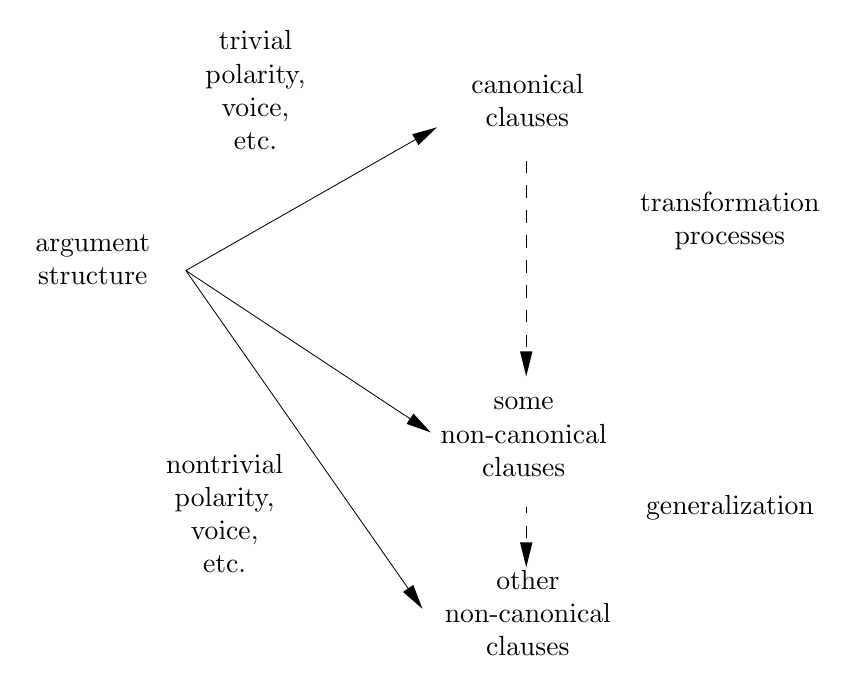
\begin{tikzpicture}[x=0.75pt,y=0.75pt,yscale=-1,xscale=1]
%uncomment if require: \path (0,386); %set diagram left start at 0, and has height of 386

%Straight Lines [id:da13680161853786577] 
\draw    (194,152.81) -- (313.26,84.8) ;
\draw [shift={(315,83.81)}, rotate = 150.31] [fill={rgb, 255:red, 0; green, 0; blue, 0 }  ][line width=0.08]  [draw opacity=0] (12,-3) -- (0,0) -- (12,3) -- cycle    ;
%Straight Lines [id:da16837784710650316] 
\draw    (194,152.81) -- (310.33,229.71) ;
\draw [shift={(312,230.81)}, rotate = 213.47] [fill={rgb, 255:red, 0; green, 0; blue, 0 }  ][line width=0.08]  [draw opacity=0] (12,-3) -- (0,0) -- (12,3) -- cycle    ;
%Straight Lines [id:da07747924239146564] 
\draw    (194,152.81) -- (306.85,314.17) ;
\draw [shift={(308,315.81)}, rotate = 235.03] [fill={rgb, 255:red, 0; green, 0; blue, 0 }  ][line width=0.08]  [draw opacity=0] (12,-3) -- (0,0) -- (12,3) -- cycle    ;
%Straight Lines [id:da42303822011922976] 
\draw  [dash pattern={on 4.5pt off 4.5pt}]  (358,201.81) -- (358,98.15) ;
\draw [shift={(358,203.81)}, rotate = 270] [fill={rgb, 255:red, 0; green, 0; blue, 0 }  ][line width=0.08]  [draw opacity=0] (12,-3) -- (0,0) -- (12,3) -- cycle    ;
%Straight Lines [id:da4793554387643766] 
\draw  [dash pattern={on 4.5pt off 4.5pt}]  (358,293.81) -- (358,266.81) ;
\draw [shift={(358,295.81)}, rotate = 270] [fill={rgb, 255:red, 0; green, 0; blue, 0 }  ][line width=0.08]  [draw opacity=0] (12,-3) -- (0,0) -- (12,3) -- cycle    ;

% Text Node
\draw (118,134) node [anchor=north west][inner sep=0.75pt]   [align=left] {\begin{minipage}[lt]{44.93pt}\setlength\topsep{0pt}
\begin{center}
argument\\structure
\end{center}

\end{minipage}};
% Text Node
\draw (200,36) node [anchor=north west][inner sep=0.75pt]   [align=left] {\begin{minipage}[lt]{39.53pt}\setlength\topsep{0pt}
\begin{center}
trivial\\polarity,\\voice,\\etc. 
\end{center}

\end{minipage}};
% Text Node
\draw (328,57) node [anchor=north west][inner sep=0.75pt]   [align=left] {\begin{minipage}[lt]{44.05pt}\setlength\topsep{0pt}
\begin{center}
canonical\\clauses
\end{center}

\end{minipage}};
% Text Node
\draw (313,213) node [anchor=north west][inner sep=0.75pt]   [align=left] {\begin{minipage}[lt]{63.87pt}\setlength\topsep{0pt}
\begin{center}
some\\non-canonical\\clauses
\end{center}

\end{minipage}};
% Text Node
\draw (315,296) node [anchor=north west][inner sep=0.75pt]   [align=left] {\begin{minipage}[lt]{63.87pt}\setlength\topsep{0pt}
\begin{center}
other\\non-canonical\\clauses
\end{center}

\end{minipage}};
% Text Node
\draw (181,240) node [anchor=north west][inner sep=0.75pt]   [align=left] {\begin{minipage}[lt]{45.76pt}\setlength\topsep{0pt}
\begin{center}
nontrivial\\polarity,\\voice,\\etc. 
\end{center}

\end{minipage}};
% Text Node
\draw (409,114) node [anchor=north west][inner sep=0.75pt]   [align=left] {\begin{minipage}[lt]{68.79pt}\setlength\topsep{0pt}
\begin{center}
transformation\\processes
\end{center}

\end{minipage}};
% Text Node
\draw (412,260) node [anchor=north west][inner sep=0.75pt]   [align=left] {\begin{minipage}[lt]{64.45pt}\setlength\topsep{0pt}
\begin{center}
generalization
\end{center}

\end{minipage}};


\end{tikzpicture}
